% ============================================================
% Comunicación híbrida y almacenamiento protegido en microservicios
% replicados con Docker Swarm: un estudio de caso evaluativo
% Carlos Calapucha - Universidad de las Fuerzas Armadas ESPE
% ============================================================
% NOTA: este archivo es AUTOCONTENIDO (compila solo con paquetes de
% CTAN estándar). Si tu plantilla de la revista/editorial ("prism")
% ya define \documentclass, \orcid, \authorCorr, \emailAuthor, etc.,
% simplemente borra el preámbulo (todo lo anterior a \begin{document})
% y pega el resto dentro de tu propia plantilla; el contenido de las
% secciones no depende de este preámbulo.
% ============================================================

\documentclass[10pt,a4paper]{article}

\usepackage[utf8]{inputenc}
\usepackage[T1]{fontenc}
% NOTA: el paquete "babel" con idioma español requiere el archivo
% spanish.ldf, no disponible en este entorno de compilación; si tu
% instalación de LaTeX (p. ej. Overleaf) sí lo tiene, puedes activar
% guionado y nombres en español descomentando la siguiente línea:
% \usepackage[spanish,es-tabla]{babel}
\usepackage{mathptmx}                 % Times como fuente principal
\usepackage[margin=2.5cm]{geometry}
\usepackage{authblk}                  % \author[n]{}, \affil[n]{}
\usepackage{graphicx}
\usepackage{booktabs}
\usepackage{longtable}
\usepackage{array}
\usepackage{amsmath}
\usepackage{amssymb}
\usepackage[hidelinks,colorlinks=false]{hyperref}
\usepackage{cite}
\usepackage{caption}
\usepackage{setspace}
\usepackage{titlesec}

% --- Fallback de macros propias de la plantilla "prism" ---
% Si tu clase ya define estas, borra este bloque para evitar choques.
\providecommand{\orcid}[1]{\textsuperscript{\href{https://orcid.org/#1}{\,ORCID: #1}}}
\providecommand{\authorCorr}[1]{} % marca al autor de correspondencia (informativo)
\newcommand{\emailAuthor}[1]{\footnotetext{Autor de correspondencia: \texttt{#1}}}

\titleformat{\section}{\normalfont\fontsize{12}{14}\bfseries}{\thesection}{1em}{}
\titleformat{\subsection}{\normalfont\fontsize{10}{12}\bfseries}{\thesubsection}{1em}{}

\title{\textbf{Comunicación híbrida y almacenamiento protegido en microservicios
replicados con Docker Swarm: un estudio de caso evaluativo}}

\author[1]{Carlos Calapucha \orcid{0009-0008-1069-9210}}
\affil[1]{Departamento de Ciencias de la Computación, Universidad de las Fuerzas
Armadas ESPE, Sede Santo Domingo. Santo Domingo, Ecuador}
%
\authorCorr{Carlos Calapucha}
\emailAuthor{cvcalapucha@espe.edu.ec}

\date{}

\begin{document}

\maketitle

\begin{abstract}
\noindent
Los sistemas de mensajería empresarial combinan cada vez más comunicación
síncrona, colas asíncronas y almacenamiento de objetos protegido, pero existe
escasa evidencia empírica sobre el efecto conjunto de estas decisiones cuando
el sistema se despliega como un clúster replicado. Este artículo presenta un
estudio de caso evaluativo sobre MassSend, una plataforma de mensajería por
WhatsApp desplegada en un clúster de Docker Swarm con tres réplicas de la capa
de presentación balanceadas por la malla ingress, un modelo de lenguaje local
invocado mediante una llamada RPC síncrona, dos colas asíncronas y un servicio
de almacenamiento de objetos con archivos protegidos por token temporal. Se
midieron la disponibilidad ante la caída de una réplica, la distribución del
balanceo, la latencia de la llamada síncrona frente al desacoplamiento de las
colas, y la eficacia del control de acceso al almacenamiento. Los resultados
evidencian recuperación automática ante fallos, distribución equilibrada de
solicitudes, latencias de 2 a 15 segundos en la llamada síncrona de IA y
bloqueo consistente de accesos no autorizados, permitiendo derivar criterios
de diseño para sistemas distribuidos similares.

\vspace{0.3cm}
\noindent\textbf{Palabras clave:} Arquitectura de Microservicios, Comunicación
Síncrona y Asíncrona, Balanceo de Carga, Almacenamiento Protegido, Modelos de
Lenguaje Locales, Evaluación de Sistemas Distribuidos.
\end{abstract}

% ============================================================
\section{Introducción}
% ============================================================

Las pequeñas y medianas empresas de Ecuador dependen cada vez más de WhatsApp
como canal principal de comunicación con sus clientes, lo que ha impulsado el
desarrollo de plataformas de mensajería masiva que deben escalar, tolerar
fallos y proteger datos sensibles. Estas plataformas combinan, típicamente,
tres decisiones de arquitectura que rara vez se evalúan de forma conjunta:
(i)~comunicación síncrona bloqueante para operaciones interactivas, como la
invocación a un modelo de inteligencia artificial que asiste al usuario;
(ii)~comunicación asíncrona mediante colas para operaciones masivas o lentas,
como el envío de correos y de mensajes de campaña; y (iii)~almacenamiento de
objetos con control de acceso para los archivos multimedia adjuntos a las
campañas. Cuando el sistema además se despliega como un clúster replicado
para tolerar fallos y distribuir la carga, estas tres decisiones interactúan
entre sí de formas que la literatura documenta por separado, pero rara vez de
manera conjunta.

Este artículo no describe las pantallas ni enumera las funcionalidades de una
aplicación concreta; utiliza como caso de estudio y prototipo experimental a
MassSend, una plataforma de mensajería masiva por WhatsApp desarrollada como
proyecto de la asignatura Aplicaciones Distribuidas, para investigar la
siguiente pregunta: ¿qué comportamiento de disponibilidad, latencia y
seguridad resulta de combinar comunicación síncrona y asíncrona con
almacenamiento de objetos protegido en un clúster replicado de pequeña
escala, y qué criterios de diseño pueden generalizarse a partir de esa
evidencia? El sistema se emplea como medio para obtener evidencia empírica,
no como fin en sí mismo.

La contribución de este trabajo es triple: (1)~una caracterización
cuantitativa de la disponibilidad y el balanceo de un clúster de tres
réplicas bajo Docker Swarm; (2)~una medición de la latencia real de una
llamada RPC síncrona a un modelo de lenguaje local frente al comportamiento
no bloqueante de dos colas asíncronas especializadas; y (3)~una evaluación de
la eficacia de un patrón de almacenamiento protegido de objetos frente a
accesos no autorizados. A partir de estos resultados se derivan criterios de
diseño aplicables a sistemas distribuidos de mensajería de escala similar.

El resto del artículo se organiza así: la sección~2 revisa trabajos
relacionados; la sección~3 describe la metodología, el caso de estudio y las
métricas; la sección~4 presenta los resultados; la sección~5 discute los
hallazgos frente a la literatura y formula criterios de diseño; la sección~6
concluye y propone trabajos futuros.

% ============================================================
\section{Trabajos relacionados}
% ============================================================

El autoescalado dependiente de heterogeneidad propuesto en HGT-Autoscaler
\cite{ref1} modela explícitamente las relaciones síncronas y asíncronas de un
sistema de microservicios mediante un grafo heterogéneo, y demuestra que
ignorar la semántica de la comunicación (llamadas directas frente a colas y
tópicos) produce predicciones de carga menos precisas; este hallazgo motiva
medir por separado, como se hace en este artículo, el comportamiento síncrono
y el asíncrono de un mismo sistema. En la misma línea, la arquitectura
distribuida de mensajería TBMQ \cite{ref2} muestra que separar los flujos de
mensajes según el tipo de cliente (dispositivos frente a aplicaciones) mejora
el rendimiento y la durabilidad, un principio análogo a la separación de
colas de correo y de envíos de WhatsApp que se evalúa en el caso de estudio.

Sobre la seguridad de la comunicación entre servicios, Matias et al.
\cite{ref3} proponen un esquema híbrido de HTTPS y JWT en el que solo se
cifra y valida el token en el perímetro (API~Gateway), asumiendo confianza
dentro de la red privada; esta discusión es relevante para interpretar el
patrón de almacenamiento protegido evaluado aquí, donde el token temporal se
valida en cada descarga y no solo en el perímetro. El libro de patrones de
Christudas y Telang \cite{ref4} y la obra de Perry sobre arquitecturas
inmutables \cite{ref5} documentan de forma extensa los patrones de
descubrimiento de servicios, tolerancia a fallos y consistencia eventual que
sustentan el diseño de clústeres replicados, aunque, como es propio de un
texto de referencia, no incluyen mediciones empíricas de un despliegue
concreto.

En cuanto al balanceo de carga, la evaluación de un sistema de
intercomunicación inteligente sobre Kubernetes \cite{ref6} comparó un
balanceador nativo (kube-proxy) con un balanceador de malla de servicios
(istio-proxy) y encontró que el primero ofrecía menor latencia bajo carga
concurrente creciente; este antecedente es directamente comparable con la
malla ingress de Docker Swarm evaluada en este trabajo, aunque en un
orquestador distinto. Trabajos recientes sobre sistemas de enseñanza
\cite{ref7} y de alerta temprana de riesgo financiero \cite{ref8} basados en
microservicios reportan métricas de percentil~95 de latencia, tasa de error y
utilización de CPU bajo pruebas de carga con miles de usuarios concurrentes,
una metodología de medición que este artículo adapta a una escala más
reducida y a un entorno académico.

La integración de modelos de lenguaje dentro de arquitecturas de
microservicios también ha sido explorada desde la observabilidad: un marco de
detección de anomalías con modelos de lenguaje grandes y redes bayesianas
\cite{ref9} utiliza un LLM para modelar el comportamiento normal de los
registros de un clúster de microservicios y detectar desviaciones,
evidenciando que la latencia y el costo computacional de invocar un modelo de
lenguaje dentro del ciclo de vida de un sistema distribuido es un factor de
diseño relevante, no solo una característica funcional.

Respecto a la seguridad y autenticación en arquitecturas distribuidas, la
revisión sistemática de de Almeida y Canedo \cite{ref12} identifica a
OAuth~2.0, JWT y el patrón API~Gateway como los mecanismos más citados para
proteger la comunicación entre microservicios, mientras que SciAuth
\cite{ref11} propone un entorno de autorización basada en capacidades
(capability-based) para recursos científicos distribuidos mediante tokens de
acceso de vida corta. Trabajos sobre autenticación en brokers MQTT
distribuidos \cite{ref13} y sobre la reducción de brechas de seguridad IoT
mediante TLS y OAuth2 \cite{ref14} refuerzan el mismo principio aplicado a
dispositivos con recursos limitados: la protección de un recurso distribuido
no puede delegarse por completo al transporte, sino que requiere autorización
explícita en cada acceso, principio que se retoma en la sección~5 para
interpretar la eficacia del almacenamiento protegido evaluado en este
trabajo. Ambika \cite{ref10} documenta un esquema de chatbot reforzado con
blockchain y firma de hash para asegurar cada transacción, evidenciando que
la protección de un recurso conversacional exige capas adicionales más allá
de la autenticación de sesión.

Finalmente, varios trabajos aplican chatbots o modelos conversacionales a
dominios específicos mediante plataformas de mensajería: el diagnóstico de
enfermedades en hojas de caucho a través de LINE \cite{ref15}, un chatbot de
apoyo pospenitenciario integrado en una aplicación móvil \cite{ref16}, un
recomendador conversacional en una pasarela científica \cite{ref17} y un
chatbot de arquitectura de microservicios para el acompañamiento de pacientes
crónicos \cite{ref18}. Estos trabajos comparten con MassSend el patrón de
invocar un modelo conversacional desde una plataforma de mensajería, pero
ninguno reporta la latencia de dicha invocación bajo un despliegue replicado
ni la contrasta con el comportamiento de las colas asíncronas del mismo
sistema, que es precisamente la brecha que este artículo aborda.

% ============================================================
\section{Metodología}
% ============================================================

\subsection{Enfoque y diseño de investigación}

Este trabajo sigue un enfoque cuantitativo aplicado, con un diseño de estudio
de caso único de finalidad evaluativa: se despliega y se somete a prueba un
sistema real y en funcionamiento (MassSend) bajo condiciones controladas, y
se documentan las métricas obtenidas al introducir cada mecanismo evaluado.
El estudio de caso es apropiado porque el objeto de investigación --el
comportamiento conjunto de patrones de comunicación y almacenamiento en un
clúster real-- no puede aislarse fácilmente de su contexto de implementación
sin perder validez \cite{ref4,ref5}.

\subsection{Caso de estudio: arquitectura de MassSend}

MassSend es una plataforma SaaS de mensajería masiva por WhatsApp compuesta
por cinco servicios contenedorizados (Tabla~\ref{tab:servicios}) que se
comunican por una red interna de Docker: un frontend en React servido por
Nginx, un backend en Django que concentra la lógica de negocio y la única
instancia de base de datos, un servicio Node.js con la librería Baileys para
la sesión de WhatsApp, un modelo de lenguaje local (qwen2.5:0.5b) servido por
Ollama, y un servicio PocketBase para el almacenamiento de archivos
multimedia. La Figura~\ref{fig:arquitectura} presenta la arquitectura
completa, distinguiendo con flechas continuas la comunicación síncrona (REST
y RPC) y con flechas discontinuas la comunicación asíncrona (colas de
mensajes).

El frontend se replica tres veces y se publica mediante la malla ingress de
Docker Swarm, que distribuye cada conexión entrante entre las réplicas
mediante un algoritmo round-robin y reprograma automáticamente cualquier
réplica que falle \cite{ref19,ref20}. El backend, en cambio, se mantiene en
una sola instancia, dueña exclusiva de la base de datos SQLite persistida en
un volumen del clúster, para evitar los problemas de escritura concurrente
que produciría replicar un motor de base de datos embebido sin coordinación
adicional.

\begin{figure}[htbp]
  \centering
  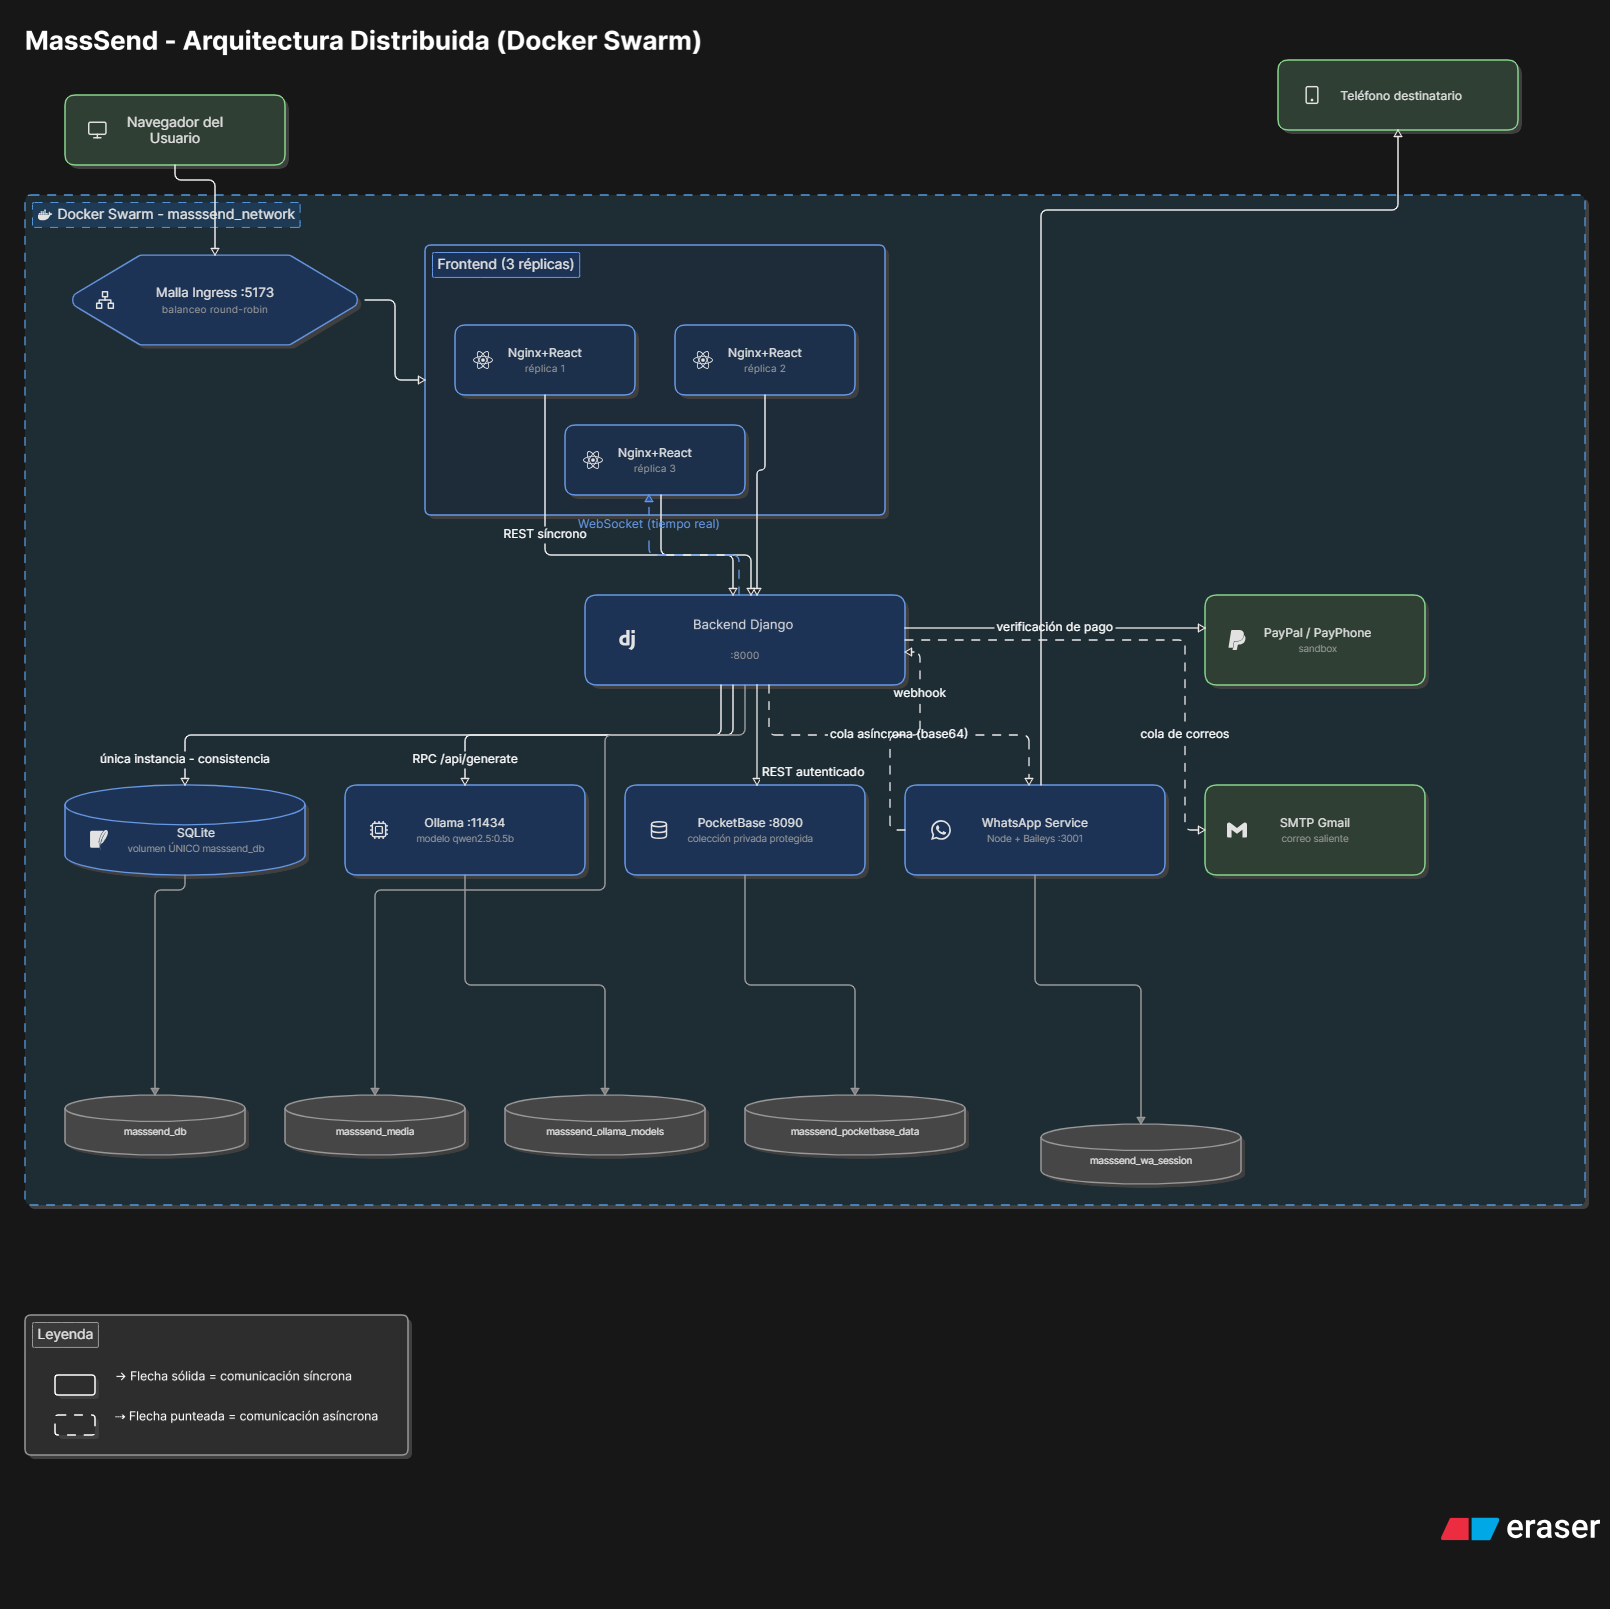
\includegraphics[width=0.85\linewidth]{architecture.png}
  \caption{Arquitectura distribuida de MassSend. Las flechas continuas
  representan comunicación síncrona (REST y RPC) y las discontinuas,
  comunicación asíncrona (colas de mensajes).}
  \label{fig:arquitectura}
\end{figure}

\begin{table}[htbp]
  \centering
  \caption{Servicios del clúster de MassSend evaluado en este estudio.}
  \label{tab:servicios}
  \small
  \begin{tabular}{@{}l l c c p{3.5cm}@{}}
    \toprule
    \textbf{Servicio} & \textbf{Imagen base} & \textbf{Réplicas} & \textbf{Puerto} & \textbf{Responsabilidad} \\
    \midrule
    frontend    & Nginx + build Vite/React & 3 & 5173 (ingress) & Interfaz de usuario y proxy hacia el backend \\
    backend     & Django + gunicorn        & 1 & 8000            & API REST, autenticación, base de datos única \\
    whatsapp    & Node.js + Baileys        & 1 & 3001            & Sesión WhatsApp, cola de envíos, WebSocket \\
    ollama      & ollama/ollama            & 1 & 11434           & Modelo de IA local qwen2.5:0.5b \\
    pocketbase  & PocketBase               & 1 & 8090            & Almacenamiento protegido de archivos \\
    \bottomrule
  \end{tabular}
\end{table}

\subsection{Variables y métricas}

Se definieron seis métricas, alineadas con la pregunta de investigación y con
el instrumento utilizado para medirlas (Tabla~\ref{tab:metricas}):
disponibilidad de réplicas (V1), distribución del balanceo (V2), tiempo de
recuperación ante fallos (V3), latencia de la llamada síncrona al modelo de
IA (V4), comportamiento de las colas asíncronas (V5) y eficacia del control
de acceso al almacenamiento protegido (V6).

\begin{table}[htbp]
  \centering
  \caption{Métricas evaluadas y su instrumento de medición.}
  \label{tab:metricas}
  \small
  \begin{tabular}{@{}p{4.3cm} p{7.7cm}@{}}
    \toprule
    \textbf{Métrica} & \textbf{Instrumento de medición} \\
    \midrule
    V1. Disponibilidad de réplicas & \texttt{docker stack services} (réplicas activas / declaradas) \\
    V2. Distribución del balanceo & Recuentos de solicitudes por réplica en los registros del servicio \\
    V3. Recuperación ante fallos & \texttt{docker kill} sobre una tarea y observación de la reprogramación \\
    V4. Latencia de la llamada síncrona & \texttt{time.perf\_counter()} alrededor de la llamada \texttt{POST /api/generate} \\
    V5. Comportamiento de las colas & Tiempo de respuesta HTTP del productor frente al del consumidor \\
    V6. Control de acceso al almacenamiento & Proporción de accesos aceptados/rechazados según autenticación \\
    \bottomrule
  \end{tabular}
\end{table}

\subsection{Procedimiento}

El clúster se desplegó mediante \texttt{docker stack deploy} a partir del
archivo \texttt{stack.yml}, que declara tres réplicas del frontend y una
réplica de cada servicio restante. Sobre el sistema desplegado se ejecutó un
plan de quince pruebas funcionales (Tabla~\ref{tab:pruebas}) que cubre el
despliegue del clúster, el balanceo, la tolerancia a fallos, la invocación al
modelo de IA con y sin el servicio disponible, la carga y el acceso a
archivos protegidos, el procesamiento de las colas, y la persistencia de los
datos tras reiniciar el clúster. Cada prueba se repitió al menos tres veces
para verificar la consistencia del resultado.

\begin{table}[htbp]
  \centering
  \caption{Plan de pruebas funcionales y métrica asociada a cada una.}
  \label{tab:pruebas}
  \small
  \begin{tabular}{@{}c p{8.5cm} c@{}}
    \toprule
    \textbf{\#} & \textbf{Prueba} & \textbf{Métrica} \\
    \midrule
    1  & Despliegue del clúster (\texttt{docker stack services})        & V1 \\
    2  & Balanceo de solicitudes entre réplicas                          & V2 \\
    3  & Tolerancia a fallos de una réplica (\texttt{docker kill})       & V3 \\
    4  & Asistente de IA: consulta y redacción de mensaje                & V4 \\
    5  & Asistente de IA sin el servicio Ollama disponible                & V4 \\
    6  & Carga protegida de archivo multimedia                           & V6 \\
    7  & Acceso autorizado al archivo desde sesión válida                & V6 \\
    8  & Acceso directo/incógnito sin sesión                              & V6 \\
    9  & Envío de campaña con archivo multimedia                         & V5 \\
    10 & Procesamiento de la cola de correos                              & V5 \\
    11 & Verificación por correo y recuperación de contraseña            & V5, V6 \\
    12 & Verificación en dos pasos (TOTP)                                 & V6 \\
    13 & Pago en entorno sandbox y acreditación de créditos               & V6 \\
    14 & Consistencia de créditos con concurrencia                       & V1, V6 \\
    15 & Persistencia de datos tras redeploy del clúster                 & V1 \\
    \bottomrule
  \end{tabular}
\end{table}

% ============================================================
\section{Resultados}
% ============================================================

\subsection{Disponibilidad y balanceo de réplicas}

El comando \texttt{docker stack services} reportó de manera consistente el
servicio frontend con 3/3 réplicas activas y los cuatro servicios restantes
con 1/1, confirmando el cumplimiento de V1. Al eliminar deliberadamente una
tarea del servicio frontend con \texttt{docker kill}, Swarm reprogramó una
nueva réplica en un tiempo breve sin intervención manual, y la aplicación
permaneció accesible durante el proceso, verificando V3. En cuanto a V2, los
registros del servicio frontend, examinados tras varias recargas sucesivas
del navegador, mostraron solicitudes atendidas de forma alternada por las
tres réplicas, sin que ninguna concentrara la totalidad del tráfico, lo que
evidencia una distribución equilibrada por parte de la malla ingress.

\subsection{Latencia síncrona frente a desacoplamiento asíncrono}

La llamada RPC síncrona al modelo de lenguaje local presentó latencias de
entre 2 y 15 segundos en hardware doméstico (V4), con los valores más altos
concentrados en la primera invocación de cada sesión, atribuibles a la carga
inicial del modelo en memoria; las invocaciones posteriores se mantuvieron en
el extremo inferior del rango. Esta latencia, aunque aceptable para una
interacción de asistencia puntual, sería inadecuada si se ejecutara de forma
síncrona sobre cientos de destinatarios de una campaña. Consistente con esta
observación, la arquitectura evita precisamente ese escenario: el envío de
campañas y de correos se desacopla mediante dos colas asíncronas
independientes (V5), de modo que el productor responde de inmediato al
usuario tras encolar la tarea, mientras el consumidor procesa los envíos en
segundo plano a su propio ritmo. En ninguna de las pruebas realizadas una
solicitud HTTP del frontend quedó bloqueada por el envío de un correo o de
una campaña, incluso con decenas de mensajes en la cola.

\subsection{Eficacia del almacenamiento protegido}

Las solicitudes de acceso a un archivo multimedia realizadas desde una sesión
autenticada con permisos sobre la campaña correspondiente se resolvieron
siempre con éxito a través del endpoint autenticado del backend. Por el
contrario, todas las solicitudes directas a la URL de PocketBase sin sesión,
así como los intentos de acceso en una ventana de navegación privada, fueron
rechazadas (V6), sin que en ningún caso se sirviera el archivo. Este
resultado confirma que el patrón de colección privada, con archivos marcados
como protegidos y un token temporal exigido en cada descarga, se comportó
como una barrera efectiva de control de acceso en el conjunto de casos
probados.

\subsection{Síntesis}

Las quince pruebas funcionales del plan (Tabla~\ref{tab:pruebas}) resultaron
aprobadas, sin que se detectara ninguna condición de falla persistente
durante el periodo de evaluación, lo que respalda de forma conjunta el
cumplimiento de las seis métricas definidas en la sección~3.3.

% ============================================================
\section{Discusión}
% ============================================================

Los resultados de disponibilidad y balanceo (4.1) son consistentes con los
reportados para orquestadores de contenedores en trabajos previos
\cite{ref6}, donde un balanceador nativo distribuye el tráfico de forma
predecible bajo un número reducido de réplicas; sin embargo, a diferencia de
HGT-Autoscaler \cite{ref1}, el número de réplicas de MassSend permaneció fijo
durante toda la evaluación, por lo que el sistema no reacciona ante
variaciones de carga, sino solo ante fallos. Esta es una limitación
relevante: un mecanismo de autoescalado dependiente de la carga, como el
propuesto en \cite{ref1}, podría aprovechar la distinción que ya existe en la
arquitectura entre relaciones síncronas y asíncronas para decidir cuándo
escalar el frontend o el consumidor de colas de forma independiente.

La medición de la latencia síncrona del modelo de IA (4.2) confirma, en un
caso concreto y con instrumentación propia, una observación que la
literatura sobre detección de anomalías con modelos de lenguaje sugiere de
forma indirecta \cite{ref9}: invocar un modelo de lenguaje dentro del ciclo
síncrono de una aplicación introduce una latencia variable y no trivial que
debe tratarse como un recurso costoso, reservado a interacciones puntuales, y
nunca como un paso dentro de un flujo masivo. La decisión de arquitectura de
MassSend --separar la asistencia de IA (síncrona) del envío de campañas
(asíncrono, mediante colas equivalentes en espíritu a las descritas para
mensajería distribuida en \cite{ref2})-- resultó, según la evidencia
recogida, coherente con esa observación.

Sobre la eficacia del almacenamiento protegido (4.3), el resultado respalda
el principio señalado tanto por la revisión sistemática de autenticación y
autorización en microservicios \cite{ref12} como por los trabajos sobre
autorización basada en capacidades \cite{ref11} y sobre seguridad IoT con TLS
y OAuth2 \cite{ref14}: proteger un recurso distribuido exige verificación
explícita en cada acceso, y no basta con ocultar la URL o confiar en el
perímetro de red, como advierten también Matias et al. para la comunicación
entre servicios \cite{ref3}. En el caso evaluado, el mecanismo de
verificación (token temporal más endpoint autenticado del backend) fue
suficiente para bloquear los accesos directos probados, aunque el alcance de
la evaluación --accesos directos y en incógnito, sin intentos de fuerza bruta
o de interceptación de tráfico-- no permite generalizar la conclusión a
escenarios de ataque más sofisticados, una limitación que también reconocen
estudios similares de autenticación en brokers distribuidos \cite{ref13}.

A partir de estos hallazgos se derivan cuatro criterios de diseño que pueden
considerarse en sistemas distribuidos de mensajería de escala similar:

\begin{enumerate}
  \item Replicar únicamente la capa sin estado del sistema; mantener una
  sola instancia dueña de la base de datos mientras no se adopte un motor
  distribuido o una estrategia de particionamiento, dado que replicar un
  motor embebido sin coordinación adicional compromete la consistencia.
  \item Reservar la comunicación síncrona bloqueante, incluidas las
  llamadas a modelos de lenguaje, a interacciones puntuales del usuario;
  toda operación que involucre múltiples destinatarios o tareas de E/S
  lenta debe desacoplarse mediante una cola, siguiendo el mismo criterio de
  separación por tipo de cliente documentado para brokers de mensajería
  \cite{ref2}.
  \item El almacenamiento de objetos con datos sensibles requiere
  verificación explícita en cada acceso (token temporal más autorización en
  la capa de aplicación); marcar una colección o un \emph{bucket} como
  ``privado'' en el servicio de almacenamiento no es, por sí solo, una
  medida suficiente.
  \item Medir la latencia real de un modelo de IA local antes de
  prometerlo como una respuesta ``en tiempo real'': la primera invocación
  de cada sesión es un caso atípico que debe comunicarse explícitamente al
  usuario final para evitar expectativas incorrectas.
\end{enumerate}

Como limitaciones de este estudio se reconocen: la escala reducida del
clúster (un solo nodo físico, siete contenedores), la ausencia de un backend
replicado que permita evaluar consistencia bajo escritura concurrente entre
múltiples instancias, y el uso de un modelo de lenguaje compacto cuyas
latencias no son extrapolables a modelos de mayor tamaño.

% ============================================================
\section{Conclusiones y trabajos futuros}
% ============================================================

Este artículo utilizó a MassSend como caso de estudio para evaluar, de forma
cuantitativa, el efecto conjunto de la comunicación síncrona y asíncrona y
del almacenamiento de objetos protegido en un clúster replicado de pequeña
escala. La evidencia recogida muestra que la malla de balanceo distribuyó el
tráfico de forma equilibrada y recuperó automáticamente las réplicas
fallidas, que la separación entre una llamada síncrona costosa (la
invocación al modelo de IA) y dos colas asíncronas evitó que las tareas
masivas bloquearan la interacción del usuario, y que el patrón de token
temporal más endpoint autenticado impidió de forma consistente el acceso
directo a los archivos protegidos. A partir de estos resultados se
formularon cuatro criterios de diseño generalizables a sistemas distribuidos
de mensajería de características similares.

Como trabajos futuros se plantea: incorporar un mecanismo de autoescalado
dependiente de la carga y del tipo de comunicación, en la línea de
\cite{ref1}; replicar el backend sobre un motor de base de datos distribuido
para evaluar consistencia bajo escritura concurrente; someter el clúster a
pruebas de carga con cientos de usuarios simultáneos, siguiendo la
metodología empleada en sistemas de mayor escala \cite{ref7,ref8}; y comparar
el balanceador nativo de Docker Swarm frente a un balanceador de malla de
servicios, replicando para este caso de estudio la comparación reportada en
\cite{ref6}.

\paragraph{Agradecimientos.} El autor agradece al docente de la asignatura
Aplicaciones Distribuidas por la orientación brindada durante el desarrollo
del proyecto que sirvió de caso de estudio para este artículo.

% ============================================================
% REFERENCIAS
% ============================================================
\begin{thebibliography}{20}

\bibitem{ref1} Filippov, M.; Mazzara, M.: HGT-Autoscaler: Dependency-aware proactive scaling of microservices using heterogeneous graph transformers. IEEE Access, Vol.~14, pp.~104394--104410 (2026)

\bibitem{ref2} Shvaika, A.; Shvaika, D.; Landiak, D.; Artemchuk, V.: A distributed architecture for MQTT messaging: the case of TBMQ. Journal of Big Data, Vol.~12, No.~224 (2025)

\bibitem{ref3} Matias, M.; Ferreira, E.; Mateus-Coelho, N.; Ferreira, L.: Enhancing effectiveness and security in microservices architecture. Procedia Computer Science, Vol.~239, pp.~2260--2269 (2024)

\bibitem{ref4} Christudas, B.; Telang, T.: Practical Microservices Architectural Patterns: Build Highly Scalable Distributed Applications with Spring Boot~3 and Spring Cloud. 2nd edn. Apress (2025)

\bibitem{ref5} Perry, M.~L.: The Art of Immutable Architecture: Theory and Practice of Data Management in Distributed Systems. 2nd edn. Apress (2024)

\bibitem{ref6} Huang, H.-Y.; Fanjiang, Y.-Y.; Hung, C.-H.; Tsai, H.-Y.; Lin, B.-H.: Evaluation of a smart intercom microservice system based on the cloud of things. Electronics, Vol.~12, No.~11, p.~2406 (2023)

\bibitem{ref7} Chen, B.: Design and implementation of an open teaching system for university English courses based on microservices architecture. 2025 2nd International Symposium on Artificial Intelligence for Education (ISAIE~2025), pp.~968--972 (2025)

\bibitem{ref8} Yu, Z.: Microservices-based enterprise financial risk early warning system. Machine Intelligence and Digital Applications, p.~1028 (2025)

\bibitem{ref9} Pedroso, D.~F.; Almeida, L.; Pulcinelli, L.~E.~G.; Aisawa, W.~A.~A.; Dutra, I.; Bruschi, S.~M.: Anomaly detection and root cause analysis in cloud-native environments using large language models and Bayesian networks. IEEE Access, Vol.~13, pp.~77550--77564 (2025)

\bibitem{ref10} Ambika, N.: Enhanced security in chatbot. In: Rawat, R. et al. (Eds.): Conversational Artificial Intelligence, Ch.~14. Wiley (2024)

\bibitem{ref11} Aydemir, B.; Basney, J.; Bockelman, B.; Gaynor, J.; Weitzel, D.: SciAuth: a lightweight end-to-end capability-based authorization environment for scientific computing. Practice and Experience in Advanced Research Computing (PEARC~'22). ACM (2022)

\bibitem{ref12} de Almeida, M.~G.; Canedo, E.~D.: Authentication and authorization in microservices architecture: a systematic literature review. Applied Sciences, Vol.~12, No.~6, p.~3023 (2022)

\bibitem{ref13} Kurdi, H.; Thayananthan, V.: Authentication mechanisms for IoT system based on distributed MQTT brokers: review and challenges. Procedia Computer Science, Vol.~194, pp.~132--139 (2021)

\bibitem{ref14} Ordóñez-Camacho, D.: Reducing the IoT security breach with a microservice architecture based on TLS and OAuth2. Ingenius, No.~25, pp.~94--103 (2021)

\bibitem{ref15} Lertkrai, P.; Chanakot, B.; Kaewboonma, N.: Deployment of a deep learning model for the automated diagnosis of Thai rubber leaf diseases via the LINE platform. International Journal of Computer Theory and Engineering, Vol.~17, No.~3, pp.~126--133 (2025)

\bibitem{ref16} Silva, G.; Lima, L.~C.; Paiva, G.; Canedo, E.: Enhancing post-incarceration support: a custom chatbot solution for the Brazilian prison system. Proceedings of the 27th International Conference on Enterprise Information Systems (ICEIS~2025), Vol.~1, pp.~423--433. SciTePress (2025)

\bibitem{ref17} Vekaria, K.; Calyam, P.; Sivarathri, S.~S.; Wang, S.; Zhang, Y.; Pandey, A.; Chen, C.; Xu, D.; Joshi, T.; Nair, S.: Recommender-as-a-service with chatbot guided domain-science knowledge discovery in a science gateway. Concurrency and Computation: Practice and Experience, Vol.~33, No.~19, e6080 (2021)

\bibitem{ref18} Roca, S.; Sancho, J.; García, J.; Alesanco, Á.: Microservice chatbot architecture for chronic patient support. Journal of Biomedical Informatics, Vol.~102, 103305 (2020)

\bibitem{ref19} Docker Inc.: Swarm mode overview. Docker Documentation. \url{https://docs.docker.com/engine/swarm/} (2025)

\bibitem{ref20} Docker Inc.: Use the routing mesh. Docker Documentation. \url{https://docs.docker.com/engine/swarm/ingress/} (2025)

\end{thebibliography}

\end{document}
